% !TEX encoding = UTF-8
% !TEX TS-program = pdflatex
% !TEX root = ../tesi.tex

%**************************************************************
\chapter{Reverse Proxy tramite NGINX sulle sandbox di HDA}
\label{cap:nginx-reverse-proxy}
\intro{Breve introduzione al capitolo}\\
In questo capitolo verrà esplicata la metodologia di reverse-proxy tra \textit{sandbox} applicative di HDA per premettere a diverse utenze esterne un accesso privato ad una singola istanza di HDA in esecuzione su un determinato \textit{host}.

\section{Introduzione ad NGINX}
NGINX è un applicativo web-server multipiattaforma ad alte prestazioni, comunemente usato come \textbf{reverse-proxy} o \textbf{load-balancer}. Nato nel 2004 e progettato per garantire un basso consumo di memoria, utilizza un approccio asincrono, basato su \textit{event}, dove le richieste vengono gestite su un singolo \textit{\gls{threadg}}. Ogni \textit{thread} worker, ovvero un processo che esegue un'elaborazione effettiva, è gestito da un \textit{thread} master, il quale lo coordina e lo controlla.\\
All'interno di Docker-Hub è presente un \textbf{repository ufficiale}, gestito dalla \textbf{Nginx Foundations}, contenente un'immagine ufficiale di NGINX basata sul sistema operativo \textbf{Alpine Linux}, ovvero una distribuzione Linux che ha fatto della leggerezza un requisito fondamentale. Come precedentemente spiegato in questo documento, il container atto al \textbf{reverse-proxy} automatizzato contenente un'immagine di NGINX è chiamato "nginxcontainer", e fa parte anch'esso della \textit{sandbox} applicativa di HDA.

\section{Logica di reverse-proxy su sandbox di HDA}
Affinchè un utente, interno od esterno alla \textit{intranet} aziendale, possa accedere al relativo container contenente l'istanza, personalizzata o meno, di HDA, è necessario che conosca il relativo \textbf{FQDN} della \textit{sandbox} applicativa di HDA alla quale si vuole accedere.\\
Un \textbf{FQDN}, acronimo di \textit{Fully Qualified Domain Name}, è un nome di dominio che specifica la \textbf{posizione assoluta} di un nodo (in questo caso, la nostra \textit{sandbox} applicativa di HDA) all'interno della gerarchia DNS. Un FQDN si distingue da un generico nome di dominio per l'\textbf{aggiunta del nome dell'\textit{host}} nel \textbf{prefisso} della stringa di dominio, in modo tale da renderla univoca. Un esempio di FQDN di un container è facilmente visibile nell'immagine esplicante l'architettura del progetto nel capitolo 4.1.\\
Nonostante l'utente \textbf{non acceda in maniera diretta} al container contenente l'istanza di HDA, l'attributo FQDN di ogni container nelle relative \textit{sandbox} è assegnato in \textbf{maniera automatica} da Docker Compose secondo la seguente logica decisa assieme all'Azienda:
\centerline{\textbf{nomecliente\_nomecontainer\_numeroistanza}}
dove:
\begin{itemize}
	\item \textbf{nomecliente} identifica il \textbf{nome della \textit{sandbox}} applicativa a cui il container appartiene. Generalmente, il nome della \textit{sandbox} è il nome del cliente stesso;
	\item \textbf{nomecontainer} identifica il \textbf{nome effettivo} del container (ex: "hdabasecontainer") interno alla \textit{sandbox} applicativa avente il nome del cliente;
	\item \textbf{numeroistanza} nell'immagine 4.1 identificato con il simbolo "\#", identifica la \textbf{quantità di istanze} simili di un determinato container sono in esecuzione contemporaneamente sulla \textit{sandbox} applicativa.
\end{itemize}
Una nomenclatura di container fissa e \textit{standardizzata}, secondo quanto deciso con l'Azienda, è di fondamentale importanza, in quanto permette di instradare le richieste provenienti dall'esterno ad una qualsiasi \textit{sandbox} applicativa di HDA.
Per capire al meglio come questo processo funziona, è doveroso fornire in primis al lettore una panoramica grafica circa il funzionamento logico, con relativa spiegazione immediatamente sottostante:
\begin{figure}[!h]     
\centering 
    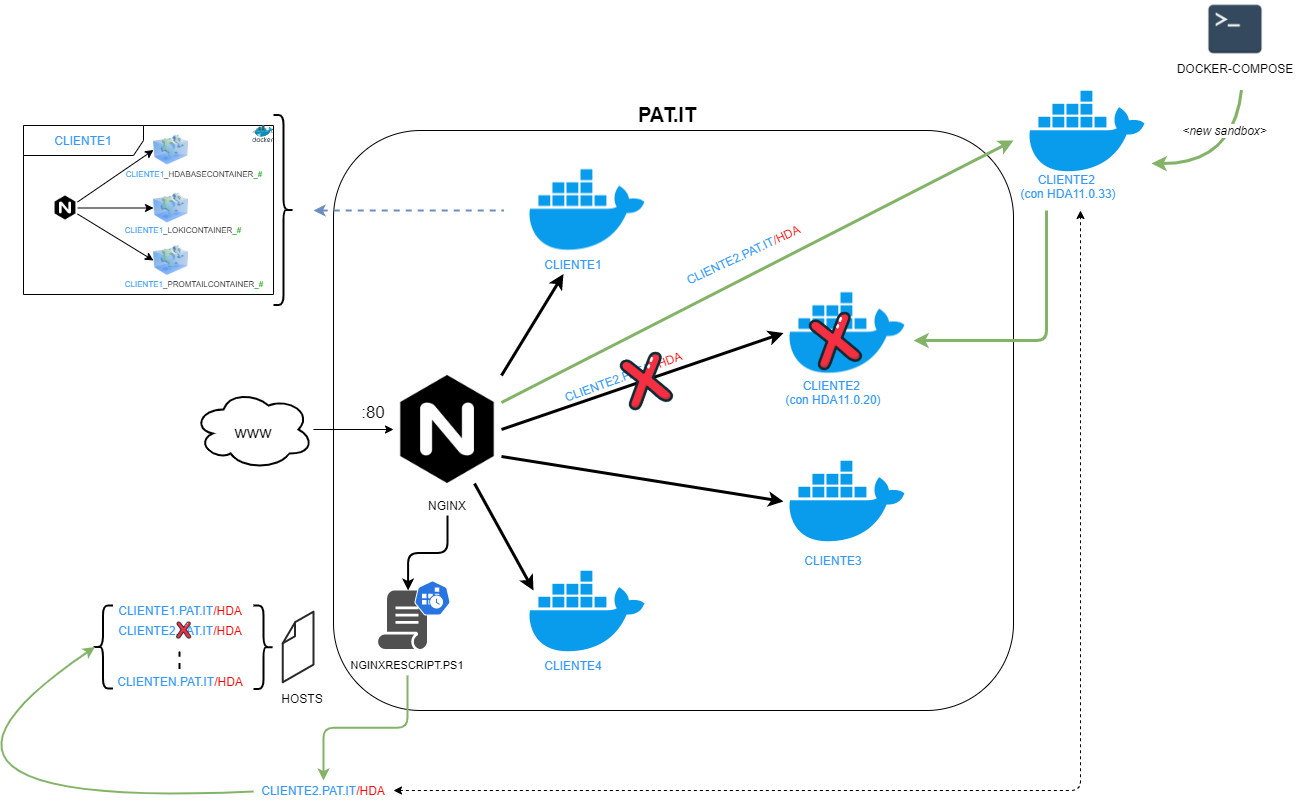
\includegraphics[width=1.0\columnwidth]{immagini/img/sandbox_nginx} 
    \caption{Rappresentazione grafica circa la gestione runtime delle \textit{sandbox} applicative di HDA}
\end{figure}\\
\newpage
Quanto sopra rappresentato, può essere facilmente riassunto nei seguenti passi:
\begin{enumerate}
	\item Arrivo della richiesta \textbf{http/https esterna} (ex: cliente1.pat.it) all'NGINX esterno configurato nell'\textbf{host \textit{PAT.IT}};
	\item Il sistema operativo dell'host \textit{PAT.IT} controlla se l'FQDN della richiesta è presente all'interno del suo \textbf{file host};%, rilevandone, se presente, l'indirizzo IP della \textit{sandbox} del relativo cliente;
	\item Il webserver NGINX controlla se l'entry "cliente1.pat.it" è presente nel suo \textbf{config file} (nginx.conf) e, se presente, provvede ad \textbf{inoltrare la richiesta} alla relativa \textit{sandbox};
	\item La richiesta HTTP \textbf{arriva al webserver NGINX interno} e quindi alla relativa \textit{sandbox} avente il nome uguale al prefisso della richiesta http (ex: cliente1);
    	\item Il webserver NGINX interno alla \textit{sandbox} applicativa \textbf{inoltra la richiesta} http al container "\textbf{hdabasecontainer}" (cliente1\_hdabasecontainer\_1), permettendo quindi agli utenti dell'azienda "cliente1" il \textbf{totale accesso all'istanza di HDA} all'interno della loro relativa \textit{sandbox} applicativa;
	\item Eventuali programmi esterni di monitoring in real-time (quali, ad esempio, Grafana) possono ora essere collegati alla \textit{sandbox} applicativa semplicemente digitando nel relativo config-file (ex in Grafana: grafana.conf) l'\textbf{FQDN della relativa \textit{sandbox} da monitorare} (ex: cliente1.pat.it). Sarà compito del relativo NGINX interno alla \textit{sandbox} gestire e dirottare (tramite proprio file di configurazione nginx.conf) ai relativi container le richieste del programma di monitoring.\\
\end{enumerate}

\subsection{Analisi del file di configurazione di NGINX interno alla sandbox applicativa}
Come già precedentemente sottolineato in questo documento, il compito del web-server NGINX interno alla \textit{sandbox} è quello di \textbf{distribuire le richieste} che arrivano dall'istanza NGINX esterna ai vari container interni alla \textit{sandbox} del relativo cliente. I container con la quale NGINX comunica sono, come precedentemente accennato, il container "\textbf{hdabasecontainer}", "\textbf{lokicontainer}" e "\textbf{primtailcontainer}".
Ognuno di questi container è accessibile da remoto con l'aggiunta del relativo url, da inserire nel \textbf{suffisso} della richiesta FQDN (ex: cliente1.pat.it/HDAPortal) come segue:
\begin{itemize}
	\item \textbf{/loki}: indirizza la richiesta al container "lokicontainer";
	\item \textbf{/promtail}: indirizza la richiesta al container "promtailcontainer";
	\item \textbf{/HDAPortal}: indirizza la richiesta al container "hdabasecontainer" contenente la versione di HDA del cliente;
	\item \textbf{suffisso vuoto}: indirizza, di default, la richiesta al container "hdabasecontainer".
\end{itemize}
Il file di configurazione di NGINX (nginx.conf) contiene, staticamente, i puntamenti \textbf{DNS} ad ognuno di questi container. La corretta \textbf{associazione} tra DNS ed indirizzo IP è svolta dal \textbf{Docker Engine} in maniera del tutto \textbf{automatizzata}.\\
Si può quindi evincere che, anche in presenza di molteplici istanze di un singolo container (ex: multiple istanze del container "hdabasecontainer") per favorire il \textbf{load-balancing} del carico, le entry nel file di configurazione di NGINX relative ai DNS dei container \textbf{rimarranno uguali}, in quanto sarà compito del Docker Engine eseguire il corretto \textbf{load-balancing} e quindi la corretta distribuzione delle richieste http/https ai relativi container multipli di HDA, tenendo \textbf{inalterato} il file di configurazione dell'istanza di NGINX interna alle \textit{sandbox}.

\subsection{Aggiornamento di HDA nella sandbox applicativa}
Come precedentemente accennato in questo documento, e come rappresentato sempre nell'immagine 6.1, risulta facilmente intuibile la fattibilità di un eventuale aggiornamento di una relativa \textit{sandbox} applicativa. Per effettuare infatti un aggiornamento alla \textit{sandbox} applicativa di HDA, sarà sufficiente eseguire i seguenti passi:
\begin{enumerate}
	\item \textbf{Eliminazione} della \textit{sandbox} applicativa contenente la versione \textit{legacy} di HDA;
	\item \textbf{Creazione} delle nuove immagini dei nuovi container della futura \textit{sandbox} applicativa di HDA tramite \textit{batch-file} \textbf{HDA\_sandbox\_builder.bat};
	\item Eseguire la \textbf{migrazione manuale} di eventuali \textit{overrides} o \textit{extensions} contenuti nella cartella \textbf{App\_Data} nel relativo \textit{volume-mapping} nell'\textit{host} ("hdashared");
	\item \textbf{Avviare}, tramite comando Docker Compose, la nuova \textit{sandbox} di HDA con il \textbf{nome uguale} alla \textit{sandbox} appena sostituita.
\end{enumerate}

Una volta eseguiti questi passi, in maniera del tutto automatica, gli utenti accederanno così alla nuova istanza di HDA aggiornata, con eventuali \textit{overrides} o \textit{customizzazioni} ereditati dalla versione di HDA precedente.\\

Grazie al risolutore DNS interno a Docker ed al suo \textit{load-balancing} automatico, nel caso di necessità di aggiornamento di \textbf{molteplici container} all'interno della \textit{sandbox} applicativa di HDA, si potrà aggiornare relativamente la versione di HDA in ogni container \textbf{senza generare alcun \textit{downtime}} al cliente, semplicemente aggiornando \textbf{un container alla volta}, per permettere quindi al \textit{load-balancer} di Docker di poter inoltrare tutte le richieste http ad almeno un container attivo e funzionante di HDA. Il meccanismo di aggiornamento di multipli container all'interno di una singola \textit{sandbox} applicativa non era nei requisiti di questo stage né è stato in alcun modo testato dallo stagista durante tutto il periodo di stage. Questa possibilità di aggiornamento e di \textit{load-balancing} dei container di HDA è stata sviluppata a livello \textbf{completamente teorico} dal sottoscritto e dal proprio tutor \textbf{Ruggero Maffei} con il preziosissimo, \textit{se non essenziale}, aiuto del Sig. \textbf{Adriano Trevisan}.

\section{Analisi NginxREScript.ps1}
Nel caso in cui il lancio o rimozione di \textit{sandbox} applicative possa essere molto frequente, per evitare all'utente installatore la continua modifica dell'\textit{host} file e del file di configurazione di NGINX, è stato predisposto uno script automatizzato che modifica, ad ogni sua esecuzione, il config file dell'\textbf{istanza di NGINX esterna} alle \textit{sandbox} applicative ed il \textbf{file host del server} dove è installata l'architettura (ex: PAT.IT).\\
Questo script Powershell, tramite interrogazione delle \textbf{Docker API}, è in grado di rilevare ogni \textit{sandbox} applicativa di HDA in esecuzione nell'\textit{host} generando, in maniera dinamica, il file di configurazione dell'istanza di NGINX (nginx.conf) esterna alle \textit{sandbox} per permettere il corretto puntamento, e quindi una corretta connessione da parte degli utenti, alle nuove \textit{sandbox} applicative appena create, o dismettere i vecchi puntamenti alle \textit{sandbox} obsolete od eliminate. 
Un flow-chart riassuntivo, per motivi di spazio, relativo allo script Powershell "\textbf{nginxREscript.ps1}" è il seguente:
\begin{figure}[!h]     
\centering 
    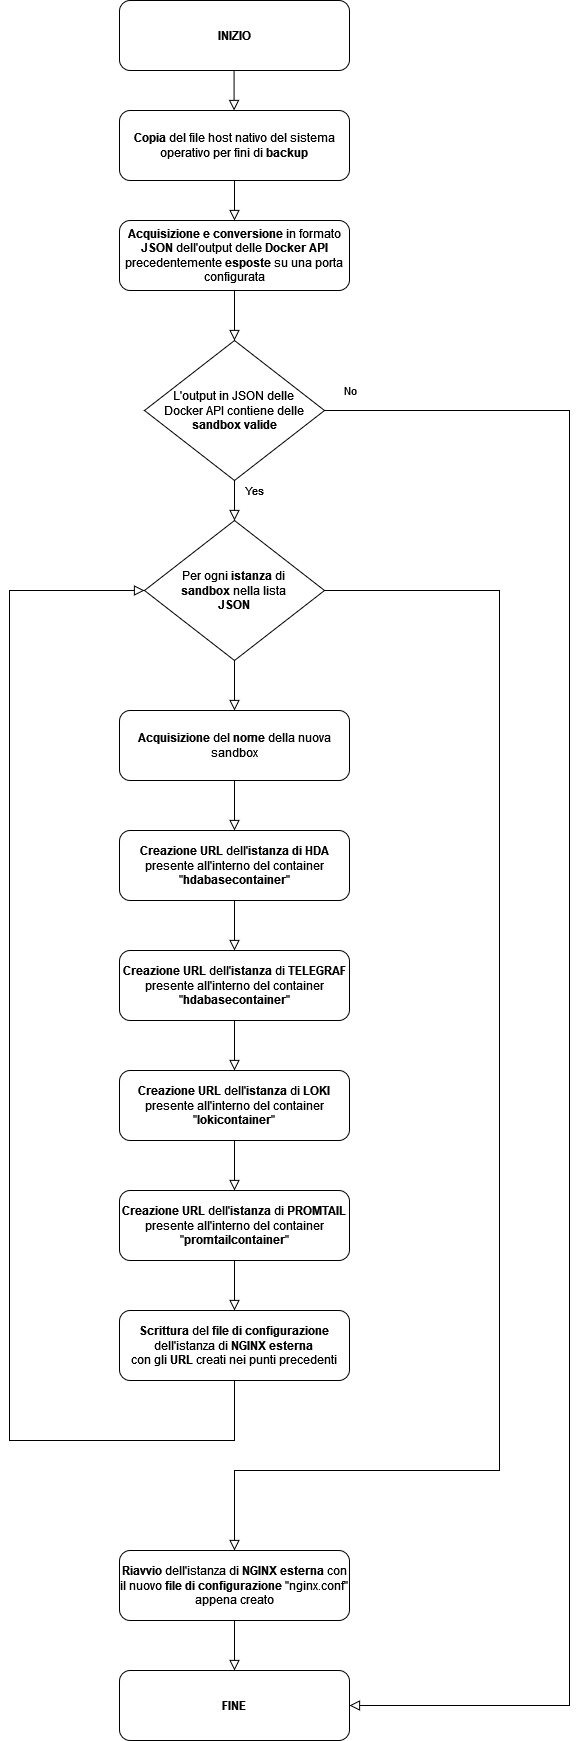
\includegraphics[width=0.45\columnwidth]{immagini/flowchart/flowchart_nginxREscript} 
    \caption{Flowchart riassuntivo relativo allo script Powershell nginxREscript.ps1}
\end{figure}\\









%**************************************************************